
\begin{figure}[H]	
\graphicspath{ {images/} }
    	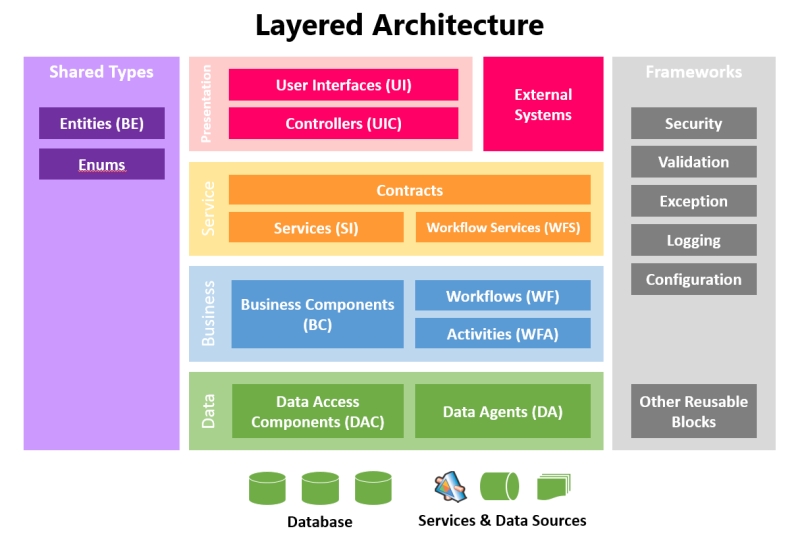
\includegraphics[scale=0.5]{layered.png}
    	\caption{Layered Architecture }
	\end{figure}
\subsection*{Layered Architecture}

System will be separated through layers; there will be User Interface  layer, services layer and process layer which includes Business logic and data. User Interface layer will handle interaction like receiving input from users, the service layer will provide the human layer with services like opening a buzz space and commenting on the buzz thread and lastly process layer will process services rendered for authorization and quality check like plagiarism. Separation through layers will enhance performance, manageability and reusability.

\begin{figure}[H]	
\graphicspath{ {images/} }
    	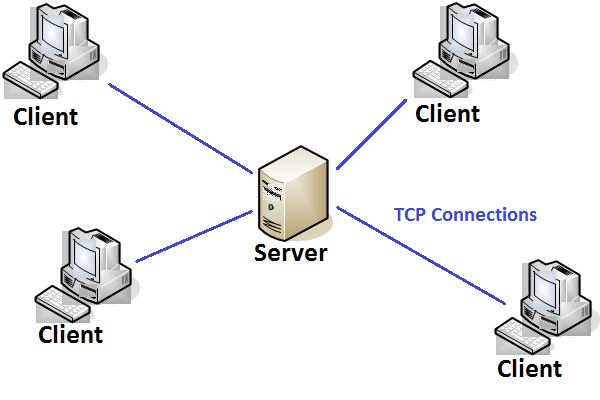
\includegraphics[scale=0.5]{csp.png}
    	\caption{Client/Server}
	\end{figure}
	
\subsection*{Client/Server} 
For communication of the server which is buzz system with users, this pattern have benefits of security as all data will be stored on the buzz system server and ease of maintenance as server is responsible of repair with client knowing of damage.


\subsection*{Model-View-Controller (MVC)}

\begin{flushleft}

Adhering to the MVC design pattern provides us with numerous benefits:

\begin{enumerate}
	\item \textbf{Separation of design concerns:} Because of the decoupling of presentation, control, and data persistence and behavior, the application becomes more flexible; modifications to one component have minimal impact on other components.
	\item \textbf{More easily maintainable and extensible:} Good structure can reduce code complexity. As such, code duplication is minimized.
	\item \textbf{Promotes division of labour:}Developers with different skill sets are able to focus on their core skills and collaborate through clearly defined interfaces.
\end{enumerate}

	\begin{figure}[H]
		\centering\graphicspath{ {images/} }
		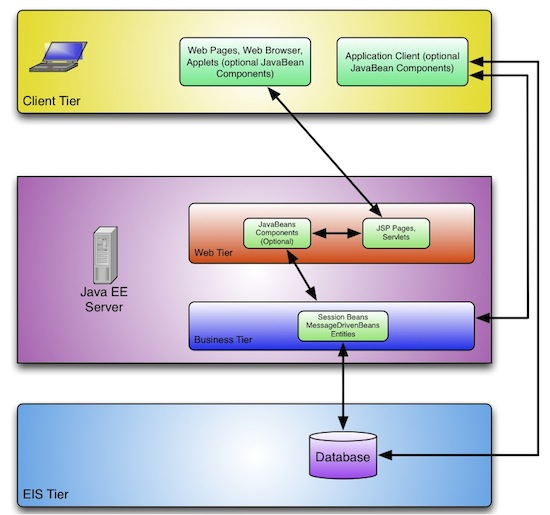
\includegraphics[width=\textwidth, height=15cm]{MVC.jpg}
	   	\caption{Java-EE system architecture}.
	\end{figure}

The system will be designed using the MVC architectural pattern combined
with a multi-tier/layered architectural pattern to form what is known as the Java-EE system architecture.
This will allows the user to be decoupled from the server and the view, the controller and the model each 
to have their own set of layers as described below.

\textbf{View (Client Tier)}\\
This tier runs on the user system and encapsulates the various components that a user system may use to access the Java EE server-side tiers. These components include dynamic web pages, Java applications and Java applets. 

\textbf{Controller (Java-EE server)}

The middle tier's business functions handle client requests and process application data, storing it in a permanent data store in the data tier.

\begin{itemize}
	\item \textbf{Web Tier}
	\\The web tier consists of components that handle the interaction between clients and the business tier.
	
	\item \textbf{Business Tier}
	\\The business tier consists of components that provide the business logic for an application. Business logic is code that provides functionality to a particular business domain.
\end{itemize}

\textbf{Model (Enterprise Information Systems (EIS) Tier)}\\
The EIS tier consists of database servers, enterprise resource planning systems, and other legacy data sources. These resources typically are located on a separate machine than the Java EE server, and are accessed by components on the business tier.

\end{flushleft}

\subsection*{Dependency Injection}

\begin{flushleft}

Dependency injection implements inversion of control for software libraries, where the caller delegates to an external framework the control flow of discovering and importing a service or software module.\\
The benefits include are creating new objects using dependencies, decoupling of code, makes code cleaner, easier to modify and easier to reuse. 
\end{flushleft}


